\newpage
\section{Derivata temporale di integrali su domini dipendenti dal tempo: formule di Leibniz}\label{sec:richiami:leibniz}
In questa sezione si enunciano e dimostrano i teoremi per la derivazione in tempo su domini mobili di integrali di volume, flussi e circuitazioni.
%In questa sezione si ricavano delle identità vettoriali che coinvolgono le derivate temporali di integrali su domini dipendenti dal tempo. In particolare si rivisita il teorema di Reynolds per la derivata temporale di integrali su volumi dipendenti dal tempo e si ricavano le formule per le derivate temporali del flusso attraverso una superficie mobile e della circuitazione di un campo vettoriale (come caso particolare di una formula per un più generale integrale su una curva aperta). La trattazione qui riportata è frutto di un compromesso tra il rigore matematico e una comprensione più immediata dell'origine dei termini che compaiono nelle formule e del loro significato fisico.
 
\begin{theorem}[Integrale di volume (Teorema di Reynolds)]\label{thm:reynolds}
%
%\begin{fBox}
\begin{equation}
  \frac{d}{dt}\int_{V(t)} f = 
  \int_{V(t)} \frac{\partial f}{\partial t} + 
  \oint_{S(t)} f \bm{v} \cdot \bm{\hat{n}}
\end{equation}
%\end{fBox}
\end{theorem}

\begin{proof}
Il volume al tempo $t+\Delta t$ può essere pensato come la somma del volume al tempo $t$ 
 e della variazione di volume $v(t,\Delta t)$, che si riscontra nell'unione, con segno, dei volumi 
 di integrazione: formalmente ``$V(t+\Delta t)=V(t)+v(t,\Delta t)$''. Il volume elementare 
 $d v$ può essere ricavato dal prodotto scalare tra la superficie elementare (con normale uscente)
 $\bm{\hat{n}} dS$ e lo spazio infinitesimo percorso dal punto della superficie $\Delta \bm{x}=\bm{v}\Delta t$,
 trascurando gli infinitesimi di ordine superiore:
 $dv = \bm{\hat{n}}\cdot \bm{v} \Delta t dS$, cfr. figura \ref{fig:vol}. Infine è possibile usare l'espansione di serie
 $f(\bm{x},t+\Delta t) = f(\bm{x},t) + \partial f / \partial t (\bm{x},t) \Delta t$.
 Si scrive l'incremento dell'integrale di volume:
\begin{equation}
\begin{aligned}
 &  \int_{V(t+\Delta t)} f(\bm{x},t+\Delta t) -  \int_{V(t)} f(\bm{x},t) = \\
 & \qquad =   \int_{V(t)} \left[ f(\bm{x},t+\Delta t) -  f(\bm{x},t) \right]
            + \int_{v(t)}        f(\bm{x},t+\Delta t) = \\
 & \qquad =  \int_{V(t)} \dfrac{\partial f}{\partial t}(\bm{x},t) \Delta t
            + \oint_{S(t)} f(\bm{x},t+\Delta t)\bm{v}(\bm{x},t) \cdot \bm{\hat{n}} \Delta t
\end{aligned}
\end{equation}
Dividendo per $\Delta t$, nel limite $\Delta t \rightarrow 0$ è possibile riconoscere a sinistra dell'uguale
 la derivata desiderata e scrivere:
\begin{equation}
  \frac{d}{dt}\int_{V(t)} f(\bm{x},t) = 
  \int_{V(t)} \frac{\partial f}{\partial t}(\bm{x},t) + 
  \oint_{S(t)} f(\bm{x},t) \bm{v}(\bm{x},t) \cdot \bm{\hat{n}}
\end{equation}
\end{proof}
%
%\begin{remark}
%La quantità
% $f$ può essere una quantità scalare, vettoriale o tensoriale.
%\end{remark}
%
\vspace{-0.5cm}
\begin{figure}[h]%[][h!]%[h!]
 \centering
 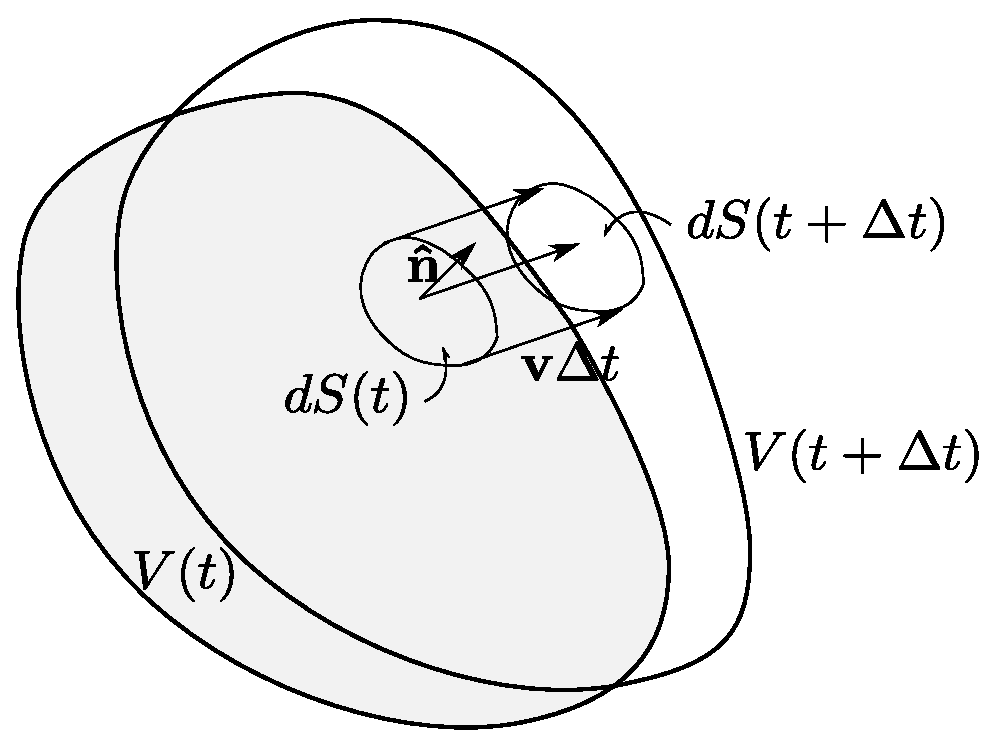
\includegraphics[width=0.48\textwidth]{./fig/vol.eps}
 \caption{Schema che illustra il moto della volume $V$, tra gli istanti temporali $t$ e 
          $t+\Delta t$. Il volume $V$ ha come frontiera la superficie esterna $S$. Viene
          messo in evidenza un elemento infinitesimo $dS$ della superficie $S$ e viene
          descritta la sua evoluzione. Si osservi la convenzione del versore normale $\bm{\hat{n}}$,
          uscente dalla superficie $S$. Il volume si muove all'interno di un dominio nel quale è
          definito il campo $f(\bm{x},t)$, non rappresentato in figura.}
\label{fig:vol}
\end{figure} 

% ++++++++++++++++++++++++++++++++++++++++++++++++++++++++++++++++++++++++++++++
\newpage
%\subsubsection{Flusso}
\begin{theorem}[Derivata temporale del flusso]
%\begin{fBox}
\begin{equation}
  \frac{d}{dt}\int_{S(t)} \bm{f}\cdot{\bm{\hat{n}}} = 
  \int_{S(t)} \left[\frac{\partial \bm{f}}{\partial t} +
  (\bm{\nabla}\cdot\bm{f}) \bm{v} \right] \cdot{\bm{\hat{n}}}  + 
  \oint_{\gamma(t)} \bm{f} \times \bm{v} \cdot \bm{\hat{t}}
\end{equation}
%\end{fBox}
\end{theorem}

\begin{proof}
Si procede in maniera analoga a quanto fatto in precedenza per l'integrale di volume. Per ricavare l'identità è richiesta
 la ``sufficiente regolarità'' del campo, poichè viene utilizzato il teorema della divergenza. Si scrive l'incremento
 del flusso
\begin{equation}
\begin{aligned}
  & \int_{S(t+\Delta t)} \bm{f}(\bm{x},t + \Delta t) \cdot \bm{\hat{n}} -   \int_{S(t)} \bm{f}(\bm{x},t) \cdot \bm{\hat{n}} = \\
  & \qquad  =  \int_{S(t+\Delta t)} \dfrac{\partial \bm{f}}{\partial t} \cdot \bm{\hat{n}} + \int_{S(t+\Delta t)} \bm{f}(\bm{x},t) \cdot \bm{\hat{n}}
   -   \int_{S(t)} \bm{f}(\bm{x},t)  \cdot \bm{\hat{n}}
\end{aligned}
\label{eqn:fl_1}
\end{equation}

Facendo riferimento alla figura \ref{fig:flux}, si applica
 il teorema della divergenza al volume (volume elementare $dv = dS(t) \bm{\hat{n}} \cdot \bm{v} \Delta t$)
 delimitato dalle superfici $S(t+\Delta t)$, $S(t)$ e dalla superficie laterale $S_{lat}$,
 che ha per elemento di superficie $\bm{\hat{n}}d S_{lat} = dl \bm{\hat{t}} \times \bm{v} \Delta t$, da considerarsi con segno, e si ottiene
\begin{equation}
  \int_{S(t+\Delta t)} \bm{f}(\bm{x},t) \cdot \bm{\hat{n}}
   -   \int_{S(t)} \bm{f}(\bm{x},t)  \cdot \bm{\hat{n}} + \oint_{\gamma(t)} \bm{f} \cdot \bm{\hat{t}} \times \bm{v} \Delta t =
  \int_{S(t)} (\bm{\nabla} \cdot \bm{f}) \bm{v} \cdot \bm{\hat{n}} \Delta t
\label{eqn:el_div}
\end{equation}
Si rielaborano i termini in (\ref{eqn:el_div}) usando la proprietà ciclica del prodotto misto
 $\bm{a} \cdot \bm{b}\times\bm{c} = \bm{c} \cdot \bm{a}\times\bm{b} = 
 \bm{b} \cdot \bm{c}\times\bm{a}$ e le proprietà del prodotto vettoriale. Si sostituisce poi in (\ref{eqn:fl_1}), si divide per $\Delta t$ e 
 si riconosce la derivata cercata facendo tendere al limite $\Delta t \rightarrow 0$, concludendo così la dimostrazione:
 \begin{equation}
   \frac{d}{dt}\int_{S(t)} \bm{f}\cdot{\bm{\hat{n}}} = 
  \int_{S(t)} \left[\frac{\partial \bm{f}}{\partial t} +
  (\bm{\nabla}\cdot\bm{f}) \bm{v} \right] \cdot{\bm{\hat{n}}}  + 
  \oint_{\gamma(t)} \bm{f} \times \bm{v} \cdot \bm{\hat{t}}
 \end{equation}
\end{proof}

\vspace{-0.5cm}
\begin{figure}[h]%[][h!]
 \centering
 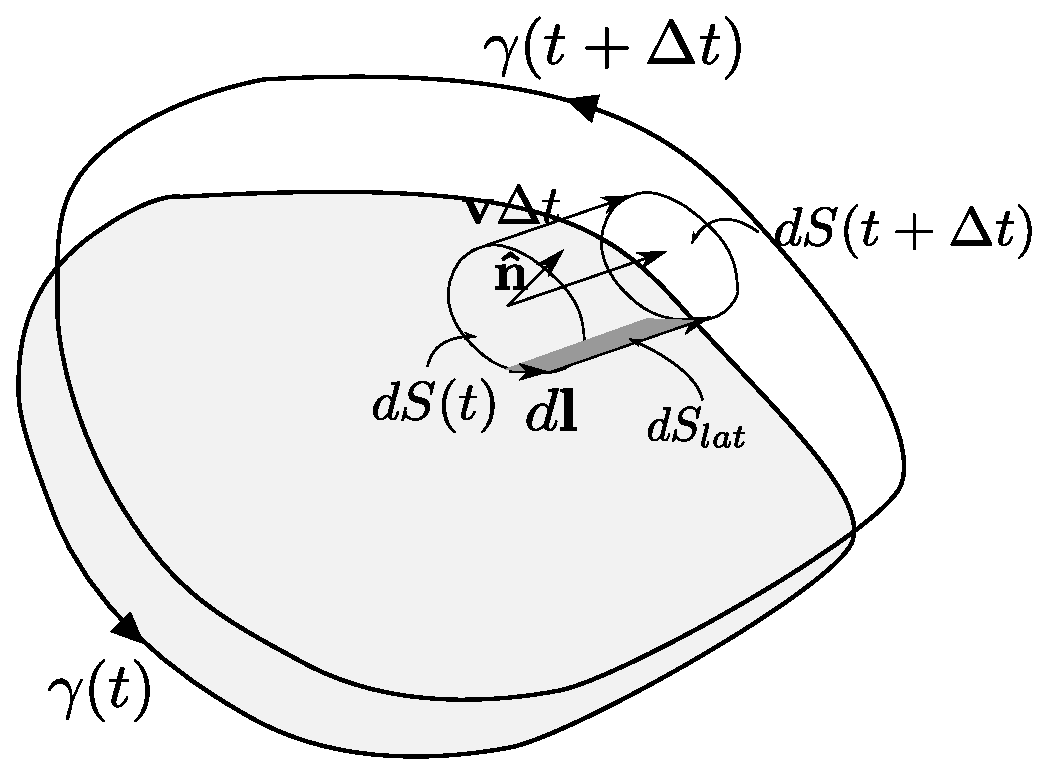
\includegraphics[width=0.50\textwidth]{./fig/flux.eps}
 \caption{Schema che illustra il moto della superficie $S$, tra gli istanti temporali $t$ e 
        $t+\Delta t$. La superficie $S$ ha come frontiera la curva $\gamma$.
        Vengono messi in evidenza l'elemento di superficie $\bm{\hat{n}}dS$,
        l'elemento di superficie laterale $\bm{\hat{n}}_{lat} dS_{lat} = 
        d\bm{l}\times \bm{v}\Delta t$ del volumetto infinitesimo $dv$. 
        Si osservi la convenzione che lega il verso di percorrenza della 
        frontiera $\gamma$ con la normale $\bm{\hat{n}}$ alla superficie
        tramite la regola della mano destra. La superficie si muove 
        all'interno di un dominio nel quale è definito il cmapo
        $\bm{f}(\bm{x},t)$, non rappresentato in figura.}
\label{fig:flux}
\end{figure} 

% ++++++++++++++++++++++++++++++++++++++++++++++++++++++++++++++++++++++++++++++
\newpage
%\subsubsection{Circuitazione}
\begin{theorem}[Derivata temporale della circuitazione]
%\begin{fBox}
\begin{equation}
  \frac{d}{dt}\int_{\gamma(t)} \bm{f}\cdot\bm{\hat{t}} = 
  \int_{\gamma(t)} \left[ \frac{\partial \bm{f}}{\partial t} + 
  (\bm{\nabla}\times\bm{f})\times\bm{v} \right]\cdot\bm{\hat{t}} +
  \bm{f}\cdot\bm{v}\bigg|_A^B
\end{equation}
%\end{fBox}
\end{theorem}
%
\begin{proof}
Seguendo un procedimento analogo a quello svolto finora si scrive l'incremento dell'integrale desiderato. Per ricavare 
 l'identità è richiesta la ``sufficiente regolarità'' del campo, poichè viene utilizzato il teorema del rotore. \vspace{-0.3cm}
\begin{equation}
\begin{aligned}
  & \int_{\gamma(t+\Delta t)} \bm{f}(\bm{x},t + \Delta t) \cdot \bm{\hat{t}} -   \int_{\gamma(t)} \bm{f}(\bm{x},t) \cdot \bm{\hat{t}} = \\
  & \qquad  =  \int_{\gamma(t+\Delta t)} \dfrac{\partial \bm{f}}{\partial t} \cdot \bm{\hat{t}} +
       \int_{\gamma(t+\Delta t)} \bm{f}(\bm{x},t) \cdot \bm{\hat{t}}
   -   \int_{\gamma(t)} \bm{f}(\bm{x},t)  \cdot \bm{\hat{t}}
\end{aligned}
\label{eqn:ci_1} \vspace{-0.3cm}
\end{equation} 
%
Facendo riferimento alla figura \ref{fig:circ}, si applica il teorema della rotore alla superficie (superfice elementare $\bm{\hat{n}}dS = dl \bm{\hat{t}} \times \bm{v} \Delta t$)
 delimitata dalle curve $\gamma(t+\Delta t)$, $\gamma(t)$ e dalle curve ``laterali''
 $\Delta\bm{x}_A = \bm{v}_A \Delta t$,  $\Delta \bm{x}_B = \bm{v}_B \Delta t$, da considerarsi con segno, e si ottiene  \vspace{-0.3cm}
\begin{equation}
  -\int_{\gamma(t+\Delta t)} \bm{f}(\bm{x},t) \cdot \bm{\hat{t}} +  \int_{\gamma(t)} \bm{f}(\bm{x},t)  \cdot \bm{\hat{t}} +
  \bm{f}(\bm{x}_B,t)\cdot\bm{v}_B \Delta t -  \bm{f}(\bm{x}_A,t)\cdot\bm{v}_A \Delta t =
  \int_{\gamma(t)} (\bm{\nabla} \times \bm{f}) \cdot \bm{\hat{t}} \times \bm{v} \Delta t
\label{eqn:el_rot}\vspace{-0.5cm}
\end{equation}
%
Si rielaborano i termini in (\ref{eqn:el_rot}) usando la proprietà ciclica del prodotto misto
 $\bm{a} \cdot \bm{b}\times\bm{c} = \bm{c} \cdot \bm{a}\times\bm{b} = 
 \bm{b} \cdot \bm{c}\times\bm{a}$ e le proprietà del prodotto vettoriale. Si sostituisce poi in (\ref{eqn:ci_1}), si divide per $\Delta t$ e 
 si riconosce la derivata cercata facendo tendere al limite $\Delta t \rightarrow 0$, concludendo così la dimostrazione:
\begin{equation}
\frac{d}{dt}\int_{\gamma(t)} \bm{f}\cdot\bm{\hat{t}} = 
  \int_{\gamma(t)} \left[ \frac{\partial \bm{f}}{\partial t} + 
  (\bm{\nabla}\times\bm{f})\times\bm{v} \right]\cdot\bm{\hat{t}} +
  \bm{f}\cdot\bm{v}\bigg|_A^B 
\end{equation}
Se il campo $\bm{f}$ e la curva $\gamma(t)$ sono continui e la curva $\gamma(t)$ è chiusa, i termini di contorno si annullano.
 Si ottiene così la derivata della circuitazione
\begin{equation}
\frac{d}{dt}\oint_{\gamma(t)} \bm{f}\cdot\bm{\hat{t}} = 
  \oint_{\gamma(t)} \left[ \frac{\partial \bm{f}}{\partial t} + 
  (\bm{\nabla}\times\bm{f})\times\bm{v} \right]\cdot\bm{\hat{t}}
\end{equation}
\end{proof}
\vspace{-1cm}
%}
\begin{figure}[h]%[h!]
 \centering
 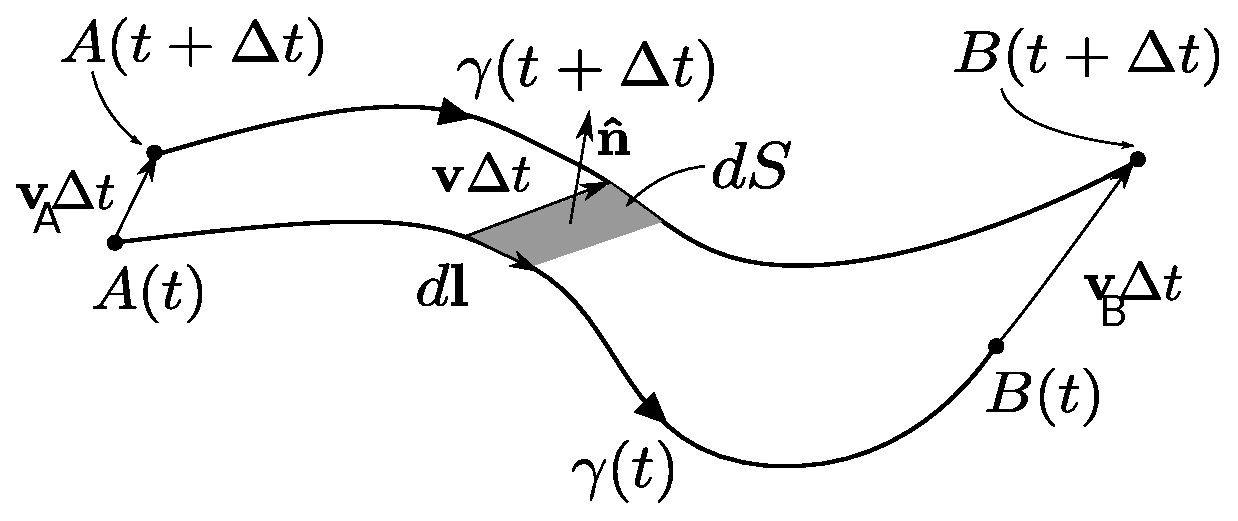
\includegraphics[width=0.5\textwidth]{./fig/circ.eps}
 \caption{Schema che illustra il moto della curva $\gamma$, tra gli istanti temporali $t$ e 
          $t+\Delta t$. La curva $\gamma$ ha come frontiera i punti $A(t)$ e
          $B(t)$. Vengono messi in evidenza l'elemento di lunghezza
          $d\bm{l} = \bm{\hat{t}} dl$ e l'elemento di superficie tra le due
          curve $\bm{\hat{n}}dS = d\bm{l} \times \bm{v} \Delta t$.
          Si osservi che per applicare il teorema del rotore con la normale
          scelta in figura, è necessario invertire il verso di percorrenza
          (e di conseguenza i segni degli integrali, cfr. eq.
          \ref{eqn:el_rot})
          della curva $\gamma(t+\Delta t)$ e del segmento elementare
          $\bm{v}_A \Delta t$, al fine di rispettare la convenzione dettata
          dalla regola della mano destra che lega la normale a una superficie
          e il verso di percorrenza della sua frontiera (cfr. figura 
          \ref{fig:flux}). La curva si muove all'interno di un dominio nel
          quale è definito il campo $\bm{f}(\bm{x},t)$, non rappresentato
          in figura.}
\label{fig:circ}
\end{figure} 


% exercises -----
\begin{exercise}
 Convincersi della validità del teorema di Reynolds, calcolandone i termini ai due lati dell'uguale, dati
 il campo scalare
 \begin{equation}
  f(x,y,t) = x \bm{\hat{x}} + t \bm{\hat{y}} \ ,
 \end{equation} 
 e il dominio rettangolare variabile nel tempo, $V(t) = [x_0(t),x_1(t)]\!\times\![y_0(t),y_1(t)]$, con 
 \begin{equation}
 \begin{aligned}
  x_0(t) = \overline{x}_0 + u_0 t \qquad & , \qquad   x_1(t) = \overline{x}_1 + u_1 t \\
  y_0(t) = \overline{y}_0 + v_0 t \qquad & , \qquad   y_1(t) = \overline{y}_1 + v_1 t \ .
 \end{aligned}
 \end{equation}
\end{exercise}

\begin{exercise}
 Dimostrare che la formula per la derivata di un integrale monodimensionale con estremi dipendenti
 dal tempo,
\begin{equation}
 \dfrac{d}{d t} \int_{a(t)}^{b(t)} f(x,t) dx = 
 \int_{a(t)}^{b(t)} \dfrac{\partial f}{\partial t}(x,t) dx + 
 f(b(t),t) \dfrac{d b}{d t}(t) - f(a(t),t) \dfrac{d a}{d t}(a) \ ,
\end{equation}
 corrisponde alla versione monodimensionale del teorema di Reynolds.
\end{exercise}

 
\newpage
